\documentclass[12pt]{article}

\usepackage{graphicx,color,enumerate,multicol}
\usepackage[top=1in,bottom=0.8in,left=1in, right=1in]{geometry}

\usepackage{rotating}
\usepackage{tikz}

\usepackage[colorlinks=true]{hyperref}

%% Use Minion fonts if available.  Otherwise Times.
\IfFileExists{MinionPro.sty}{\usepackage[lf]{MinionPro}}{}
\usepackage{amsmath,amsthm,amsbsy}
\IfFileExists{MinionPro.sty}{}{\usepackage{times,txfonts}}

%% Setup aproblem environment, 
%% aproblem items
%% subproblems environment
%% subproblem items
\makeatletter
\newcounter{probcount}
\newcounter{subprobcount}
\newlength\probsep
\newlength\pshrinking
\newif\iffirstprob
\newenvironment{aproblems}%
  {\ifhmode\unskip\par\fi\setcounter{probcount}{0}\probsep\parskip
  \sbox\@tempboxa{\textbf{9.}}\pshrinking\wd\@tempboxa\advance\pshrinking\labelsep
  \let\hproblem\aproblem
  \advance\linewidth -\pshrinking
  \advance\@totalleftmargin\pshrinking
  \advance\leftskip\pshrinking}%
  {\ifhmode\unskip \par\fi\advance\leftskip-\pshrinking}%

\newcommand{\aproblem}{%
  \setcounter{subprobcount}{0}%
  \stepcounter{probcount}%
  \def\@currentlabel{\arabic{probcount}}%
  \ifhmode
    \unskip \par
  \fi
%  \addpenalty{-4000}%
  \iffirstprob\else\addvspace\probsep\fi
  \firstprobfalse
  \hskip -\labelwidth\hskip -\labelsep 
  \hbox to\labelwidth{\hss\textbf{\arabic{probcount}.}}\hskip\labelsep
}%

\newcommand{\subprob}{\item\def\@currentlabel{\arabic{probcount}\alph{\thelistlabel}}}
\newcommand{\skipproblem}{\stepcounter{probcount}}


%% The following commands put defined left and right headers on the top, and a page number
%% on the bottom of all pages beyond page 1
\usepackage{fancyhdr}
\pagestyle{fancy}
\fancyfoot[C]{\ifnum \value{page} > 1\relax\thepage\fi}
\fancyhead[L]{\ifx\@doclabel\@empty\else\@doclabel\fi}
\fancyhead[R]{\ifx\@docdate\@empty\else\@docdate\fi}
\headheight 15pt
\def\doclabel#1{\gdef\@doclabel{#1}}
\def\docdate#1{\gdef\@docdate{#1}}
\makeatother

%% General formatting parameters
\parindent 0pt
\parskip 6pt plus 1pt


\doclabel{Math F251: After Quiz 1}
\docdate{Spring 2019}

\begin{document}
\renewcommand{\d}{\displaystyle}

\subsection*{Reminders}
\begin{itemize}
\item \textbf{Your first online homework using WebAssign ($=$ WA \S2.1 on the schedule) is due this Friday, 25 January.}  Please see the course web site for how to get started in WebAssign.
\item \textbf{Written Homework 1 ($=$ WRH 1 on the schedule) is due on Monday, 28 January at the beginning of class.}  The course web site has the assigned problems.
\end{itemize}

\subsection*{Frequently Asked Questions}
\begin{itemize}
\item \textbf{Q: When will I see my ALEKS homework grade ($=$ WRH 0) and Quiz 1 grade ($=$ proctored ALEKS assessment score plus 10 points) in Blackboard?}

A: These grades will appear on Blackboard by Friday afternoon.

\item \textbf{Q: What does my proctored ALEKS assessment score from Quiz 1 mean?}

A: The UA standard for ``calculus readiness'' is a score of 78 or higher on this proctored test.  The bar graph on the back side shows the relationship seen in the data between proctored ALEKS score and success in calculus I.  (This data is for the 550 students who took MATH 251 in Fall 2016, Fall 2017, Spring 2018, and Fall 2018.)  Regardless of your ALEKS score, to succeed you will need to work hard this semester.

\item \textbf{Q: My proctored ALEKS assessment score was low.  Will I get dropped from the class?}

A:  No. If you have already met one of the UAF prerequisites for Calculus I, you will not be
dropped for lack of prerequisite skills.  However, your instructor or an advisor may contact you if there is concern about your math placement.

\item \textbf{Q: What steps can I take now if my score was lower than I wanted?}

A: Here are some steps that you can consider taking:
    \begin{itemize}
    \item A typical student is expected to spend about 10 hours per week on calculus outside of class.  You may want to set aside in your schedule more time than that.
    \item You continue to have access to the ALEKS learning module, which can provide a structured way to continue to learn past material.
    \item You can sign up for MATH 251S, the Calculus Skills Workshop; see

\centerline{\href{https://www.uaf.edu/dms/mathlab/math-bridge/}{\texttt{www.uaf.edu/dms/mathlab/math-bridge}}}
    \item If you are worried about not being successful in calculus, UAF has made it easy for you to transfer into pre-calculus now.  You can do a drop-swap into a lower-number MATH course as late as 1 February.  Please talk to your instructor about placement, and go to the Registrar if you want to do a drop-swap.
    \end{itemize}

\item \textbf{Q: Are we done with ALEKS now or will I need to keep using it?}

A: We will not formally use ALEKS from now on, but you have 6-month access to the ALEKS Calculus I module.  You can use learning mode to improve your prerequisite skills.
\end{itemize}

\newpage

\begin{sidewaysfigure}
\begin{center}
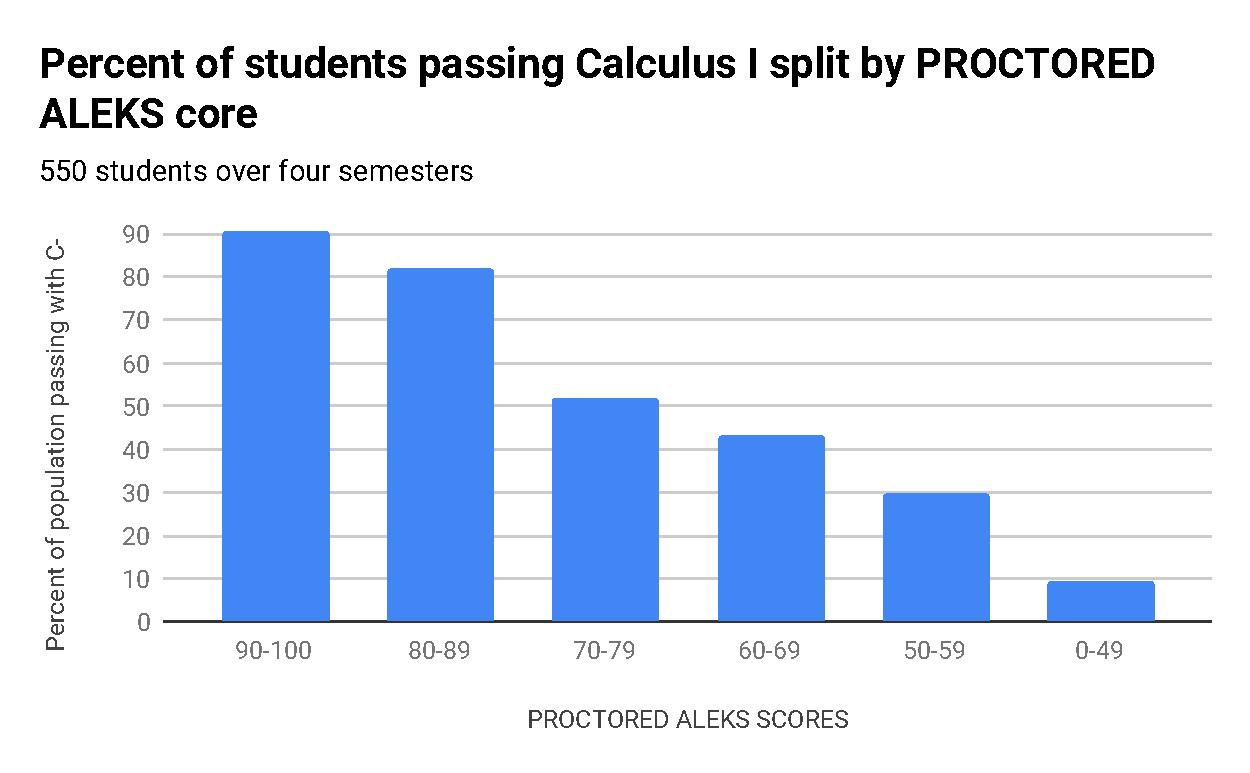
\includegraphics[width=0.95\textwidth]{ALEKS-vs-success-bar}
\end{center}
\end{sidewaysfigure}
\end{document}
